\icode{E-MD-SI-L3-261114-003}
如图所示，固定斜面倾角为 \(\theta\)，整个斜面分为 \(AB\)，\(BC\) 两段，且 \(AB = 1.5BC\)，小物块 \(P\)（可视为质点）与 \(AB\)，\(BC\) 两段斜面之间的动摩擦因数分别为 \(\mu_1\)，\(\mu_2\)，已知 \(P\) 由静止开始从 \(A\) 点释放，恰好能滑动到 \(C\) 点而停下，那么 \(\theta\)，\(\mu_1\)，\(\mu_2\) 间应满足的关系是\paren[]

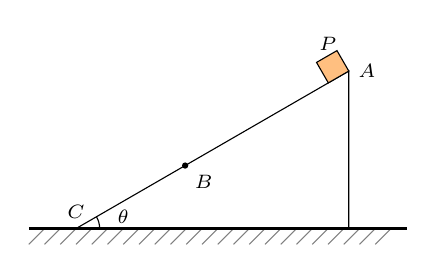
\begin{tikzpicture}[font=\scriptsize]
	\draw (0,0)node[above]{\(C\)}--(30:4)node[right]{\(A\)}--++(0,-2) (.3,0) arc(0:30:.3);
	\draw[fill=orange!50,rotate=30] (3.7,0) rectangle(4,.3);
	\node at(.6,.15){\(\theta\)};
	\foreach \x in {-.6,-.4,...,4}
		\draw[gray] (\x,-.2)--++(.2,.2);
	\draw[thick] (-.6,0)--(4.2,0);
	\fill (30:1.6)node[below right]{\(B\)} circle(.04);
	\node at(3.2,2.35){\(P\)};
\end{tikzpicture}
\begin{choices}
	\item \(\tan \theta = \dfrac{2\mu_1 + 3\mu_2}{5}\)
	\item \(\tan \theta = \dfrac{3\mu_1 + 2\mu_2}{5}\)
	\item \(\tan \theta = 2\mu_1 - \mu_2\)
	\item \(\tan \theta = 2\mu_2 - \mu_1\)
\end{choices}
\begin{answer}
    B\qquad 提示：
\end{answer}